\documentclass[
  size=12pt,
  style=sailor,
  paper=screen,
%% Try me!
%% orient=portrait,
%%  mode=handout,
%%  display=slidesnotes,
  blackslide,
  nopagebreaks,
  fleqn
]{powerdot}

\usepackage{cmap}			% Mapear caracteres especiais no PDF
\usepackage{lmodern}			% Usa a fonte Latin Modern			
\usepackage[T1]{fontenc}		% Selecao de codigos de fonte.
\usepackage[utf8]{inputenc}		% Codificacao do documento (conversão automática dos acentos)
\usepackage{listings}
\usepackage{graphicx}
\usepackage[russian, english, brazil]{babel}
\usepackage{hyperref}

\lstdefinestyle{Bash}
{language=bash,
keywordstyle=\color{blue},
basicstyle=\ttfamily,
morekeywords={peter@kbpet},
alsoletter={:~$},
morekeywords=[2]{peter@kbpet:},
keywordstyle=[2]{\color{red}},
literate={\$}{{\textcolor{red}{\$}}}1 
         {:}{{\textcolor{red}{:}}}1
         {~}{{\textcolor{red}{\textasciitilde}}}1,
}

\newcommand{\oops}[1]{\textit{#1}}

\title{Git \\ \& \\ GitHub}
\author{Alexandre Savelli Bencz}

\pdsetup{
  lf=Git \& GitHub,
  cf=\today,
  %rf=for powerdot,
  trans=Wipe,
  theslide=slide~\arabic{slide},
  list={itemsep=6pt}
}

\begin{document}

\maketitle


\begin{slide}[method=direct]{História - Git}
Desenvolvido em 2005 por Linus Torvalds, o mesmo criador do Linux, que
estava descontente com o BitKeeper, que era o sistema de controle de versão utilizado
no desenvolvimento do kernel do Linux.

\end{slide}

\section{Instalar e Configurar}

\begin{slide}[method=direct]{Instando o GIT no Linux}
	\begin{itemize}
	\item{Para instalar o Git no Ubuntu, ou em outra distribuição baseada em Debian, execute no terminal o seguinte comandos:}
		\begin{lstlisting}[style=Bash]
$ sudo apt-get install git
		\end{lstlisting}
	
		E para quem utiliza Fedora, utilize:
	
		\begin{lstlisting}[style=Bash]
$ sudo yum install git
		\end{lstlisting}
	\end{itemize}
\end{slide}

\begin{slide}[method=direct]{Configurando o GIT}
	\begin{itemize}
	\item{Sempre que instalamos o GIT, é necessario informar para o GIT, quem somos, para isto usamos as seguintes linhas de comando:
		\begin{lstlisting}[style=Bash]
$ git config --global user.name "NOME"
$ git config --global user.email E@MAIL
		\end{lstlisting}}
	\end{itemize}
\end{slide}

\section{Versionando seu código}

\begin{slide}[method=direct]{Criando um repositório}
	\begin{itemize}
		\item{Para criar e inicializar um repositório, navegue até o diretorio onde vai ficar os arquivos do seu projeto e digite o comando:
			\begin{lstlisting}[style=Bash]
$ git init
			\end{lstlisting}
		Após executar o comando, deve aparecer uma mensagem semelhante a esta:
		\begin{lstlisting}
Initialized empty Git repository in /*/.git/
		\end{lstlisting}
		}
		
		\item{Com isso já temos um repositorio, vazio, do Git inicializado, atente que o sistema criou automaticamente uma pasta chamada .git ( em modo oculto )}
	\end{itemize}
\end{slide}

\begin{slide}[method=direct]{Status do repositório}
	\begin{itemize}
		\item{Quando criamos ou adicionamos um arquivo na pasta onde foi inicializado o projeto o GIT não inclui automaticamente o novo arquivo, para isso é necessario ``rastrear'' o arquivo e adicionar ele, para isto, utilizamos o comando:
			\begin{lstlisting}[style=Bash]
$ git status
			\end{lstlisting}
			
			O resultado do comando será algo semelhante a:
			\begin{lstlisting}[basicstyle=\tiny]
$ git status
On branch master

Initial commit

Untracked files:
  (use "git add <file>..." to include in what will be committed)

        Makefile
        doc/
        fonte1.c
        fonte2.asm
        
        (...)
\end{lstlisting}
			}
	\end{itemize}
\end{slide}

\begin{slide}[method=direct]{Rastreando arquivos}
	\begin{itemize}
	\item{Para que um arquivo passe a ser rastreado pelo Git, devemos executar o seguinte comando:
		\begin{lstlisting}[style=Bash]
$ git add <nome do arquivo>
		\end{lstlisting}
	       	
	        Exemplo:
	        \begin{lstlisting}[style=Bash]
$ git add fonte2.asm
	        \end{lstlisting}
	        }
	\item{Após eecutar o comando \textit{git status} iremos ver algo semelhante com}
	\begin{lstlisting}[basicstyle=\tiny]
On branch master
Initial commit

Changes to be committed:
  (use "git rm --cached <file>..." to unstage)

        new file:   fonte2.asm

Untracked files:
  (use "git add <file>..." to include in what will be committed)

        Makefile
        (...)
	\end{lstlisting}
	\end{itemize}
\end{slide}

\begin{slide}[method=direct]{Gravando o arquivo no repo.}
	\begin{itemize}
	\item{Para gravarmos as mudanças no repositório, devemos executar o comando:
	        \begin{lstlisting}[style=Bash]
$ git commit -m ``Meu primeiro commit!!!''
	        \end{lstlisting}
	        Observe que o comando \textit{git commit} foi executado junto com o parâmetro \textit{-m}, que é utilizado para definir uma mensagem para o commit que você está submetendo ao servidor.
	        \begin{itemize}
	        \item{\textbf{A mensagem do commit deve ser muito clara, ao descrever quais são as modificações que você está enviando para o servidor!}}
	        \end{itemize}
	        Após executar o git commit, você verá:
	        \begin{lstlisting}[basicstyle=\tiny]
git commit -m "Meu primeiro commit!!!"
[master (root-commit) ff932de] Meu primeiro commit!!!
 1 file changed, 0 insertions(+), 0 deletions(-)
 create mode 100644 fonte2.asm
	         \end{lstlisting}
	        }
	\end{itemize}
\end{slide}

\begin{slide}[method=direct]{Alterando arquivos}
	\begin{itemize}
	\item{Se editarmos um arquivo já versionado pelo git, quando executamos o comando \textit{git status}, ele ira nos retornar o seguinte resultado:}
	\begin{lstlisting}[basicstyle=\tiny]
$ git status
On branch master
Changes not staged for commit:
  (use "git add <file>..." to update what will be committed)
  (use "git checkout -- <file>..." to discard changes in working directory)

        modified:   fonte2.asm
	\end{lstlisting}
	\end{itemize}
\end{slide}

\begin{slide}[method=direct]{Verificando as alterações}
	\begin{itemize}
	\item{Podemos verificar o histórico das alterações gravadas no repositório com a seguinte linha de comando:
	\begin{lstlisting}[style=Bash]
$ git log
	\end{lstlisting}
	O resultado do comando vai ser parecido com:
	\begin{lstlisting}[basicstyle=\tiny]
$ git log
commit 182279fb11c39d0830825fa0c75366c4a9905c1d
Author: Alexandre <alebencz@gmail.com>
Date:   Thu Mar 10 13:34:30 2016 -0300

    Corre<C3><A7><C3><A3>o no fonte2.asm e adicionado
    objeto para ser compilado pelo make

commit ff932ded962e4d2029eba37a879d0886036ea600
Author: Alexandre <alebencz@gmail.com>
Date:   Thu Mar 10 13:11:13 2016 -0300

    Meu primeiro commit!!!
          \end{lstlisting}
	}
	\end{itemize}
\end{slide}
\section{Compartilhando seu código pelo GitHub}

\begin{slide}[method=direct]{Git \& GitHub ?}
	\begin{itemize}
		\item{Git e GitHub são a mesma coisa?}
		\begin{itemize}
		\item{\textit{Não. Git é o sistema de controle de versões, com o qual interagimos na linha de comando. Já o GitHub é uma 					rede social para programadores que disponibiliza repositórios Git acessíveis remotamente.}}
		\end{itemize}
	\end{itemize}

	\begin{center}
	
\includegraphics[width=0.4\textwidth,natwidth=800,natheight=600]{./imagens/Octocat.png}
	\end{center}
\end{slide}

\begin{slide}[method=direct]{Criando um repositório}
	\begin{center}
	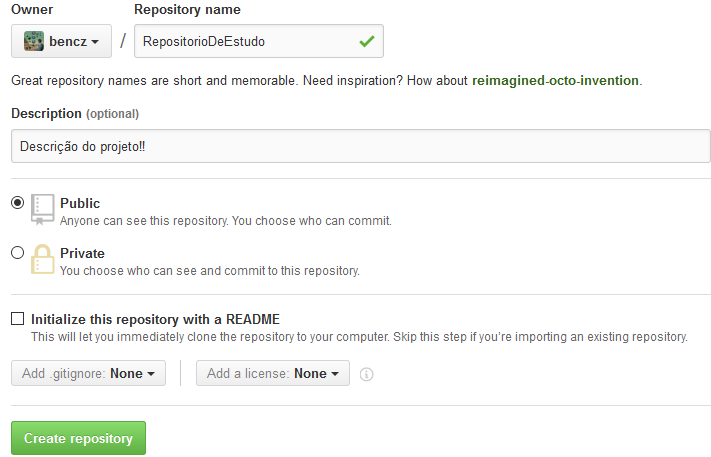
\includegraphics[width=0.9\textwidth,natwidth=711,natheight=457]{./imagens/criando_repo.png}
	\end{center}
\end{slide}

\begin{slide}[method=direct]{Apontando seu projeto para o Git}
	\begin{itemize}
	\item{Agora que já temos um repositório criado no GitHub, temos que apontar o nosso repositorio criado na nossa maquina para o repositório que foi criado no GitHub. \\
	Para isso, use o terminal e navegue até o diretorio onde está o repositorio que nós criamos e então execute a seguinte linha de comando:	}
	\end{itemize}
	
	\begin{lstlisting}[style=Bash,basicstyle=\tiny]
$ git remote add origin https://github.com/bencz/RepositorioDeEstudo.git
          \end{lstlisting}
\end{slide}

\begin{slide}[method=direct]{Enviando para o GitHub}
	\begin{itemize}
	\item{Agora que estamos com o repositório remoto configurado, podemos enviar as mudanças que fizemos para o GitHub.\\
	         Para isso, é necessario executar o comando seguinte comando:
	         \begin{lstlisting}[style=Bash]
$ git push origin master
	         \end{lstlisting}
	         Com este comando enviamos as alterações para o repositório remoto configurado com o nome \textit{origin}. \\
	         O output do comando vai ser algo semelhante com:
	         \begin{lstlisting}[style=Bash,basicstyle=\tiny]
Counting objects: 6, done.
Delta compression using up to 2 threads.
Compressing objects: 100% (3/3), done.
Writing objects: 100% (6/6), 519 bytes | 0 bytes/s, done.
Total 6 (delta 0), reused 0 (delta 0)
To https://github.com/bencz/RepositorioDeEstudo.git
 * [new branch]      master -> master
	         \end{lstlisting}
	         }
	\end{itemize}
\end{slide}

\begin{slide}[method=direct]{Clonando projetos do GitHub}
	\begin{itemize}
	\item{Para clonar um projeto do GitHub, basta utilizar o seguinte comando:
	\begin{lstlisting}[style=Bash]
$ git clone <link do projeto>.git
	\end{lstlisting}
	Quando executado o comando de clone deverá aparecer algo como:
	\begin{lstlisting}[style=Bash,basicstyle=\tiny]
$ git clone https://github.com/bencz/Beryl.git
Cloning into 'Beryl'...
remote: Counting objects: 371, done.
remote: Total 371 (delta 0), reused 0 (delta 0), pack-reused 371
Receiving objects: 100% (371/371), 69.02 KiB | 122.00 KiB/s, done.
Resolving deltas: 100% (248/248), done.
Checking connectivity... done.
	\end{lstlisting}
	}
	\end{itemize}
\end{slide}
\section{Se organizando com as branches}

\begin{slide}[method=direct]{Trabalhando em paralelo}
	\begin{itemize}
	\item{Muitos sistemas de controle de versão permite trabalho em paralelo através de \textbf{branches}}
	\item{Mas o que é uma Branch ?}
	\begin{itemize}
		\item{Uma \textbf{branch} é uma linha independente de desenvolvimento em que podemos enviar novas versões do código sem alterar as outras branches}
	\end{itemize}
	\end{itemize}
\end{slide}

\begin{slide}[method=direct]{Criando uma branch}
	\begin{itemize}
	\item{Para criar uma branch, basta executar o seguinte comando:
		\begin{lstlisting}[style=Bash]
$ git branch <nome da nova branch>
		\end{lstlisting}
		A execução deste comando não retorna nenhuma resposta, então, para listartmos as branchs existentes, utilizamos o comando:
		\begin{lstlisting}[style=Bash]
$ git branch
		\end{lstlisting}
		O resultado deste comando vai retornar a lista de todas as branchs existentes par ao projeto
		\begin{lstlisting}[style=Bash]
$ git branch
  current
* master
                   \end{lstlisting}
	         }
	\end{itemize}
\end{slide}

\begin{slide}[method=direct]{Trocando de branch}
	\begin{itemize}
	\item{Para trocarmos de uma branch para outra, executamos o seguinte comando:
	\begin{lstlisting}[style=Bash]
$ git checkout <nome da nova branch>
	\end{lstlisting}
	Quando executado este comando, deve aparecer como resposta algo como:
	\begin{lstlisting}[style=Bash]
Switched to branch 'current'
	\end{lstlisting}
	}
	\end{itemize}
\end{slide}

\begin{slide}[method=direct]{Criar e trocar para uma nova Branch}
	\begin{itemize}
	\item{Para uma questão de facilidade, o GIT fornece uma opção para criar e autoamticamente trocar de branch, quando executado o comando de checkout, o parametro \textit{-b} deve ser passado antes do nome da nova branch, executando o mesmo comando para trocar de uma branch.
	\begin{lstlisting}[style=Bash]
$ git checkout -b <nome da nova branch>
	\end{lstlisting}
	Após executar este comando, a saida será:
	\begin{lstlisting}[style=Bash]
$ git checkout -b v1.0
M       fonte2.asm
Switched to a new branch 'v1.0'
	\end{lstlisting}
	}
	\end{itemize}
\end{slide}

\begin{slide}[method=direct]{Commitando para uma branch}
	\begin{itemize}
	\item{Para commitar para uma nova branch, no momento de executar o comando \textit{push}, deve ser informado o nome da branch para qual o commit vai ser enviado:
	\begin{lstlisting}[style=Bash]
$ git push origin v1.0
	\end{lstlisting}
	Após executado o comando, o resultado será algo como:
	\begin{lstlisting}[style=Bash,basicstyle=\tiny]
$ git push origin v1.0
Counting objects: 4, done.
Delta compression using up to 2 threads.
Compressing objects: 100% (2/2), done.
Writing objects: 100% (4/4), 385 bytes | 0 bytes/s, done.
Total 4 (delta 0), reused 0 (delta 0)
To https://github.com/bencz/RepositorioDeEstudo.git
 * [new branch]      v1.0 -> v1.0
 	\end{lstlisting}
	}
	\end{itemize}
\end{slide}

\begin{slide}[method=direct]{Fazendo merge}
	\begin{itemize}
	\item{Para juntarmos as alterações feita em outras branchs com a branch \textit{master}, podemos utilizar o seguinte comando: ( Lembrando que, você deve estar na branch \textit{master} para fazer o merge com os dados da branch v1.0
	\begin{lstlisting}[style=Bash,basicstyle=\tiny]
$ git merge v1.0 -m ``Fazendo merge com a branch v1.0''
	\end{lstlisting}
	O resultado da execução deste comando será:
	\begin{lstlisting}[style=Bash,basicstyle=\tiny]
$ git merge v1.0 -m "Fazendo merge com a branch v1.0"
Updating 182279f..456bc06
Fast-forward (no commit created; -m option ignored)
 fonte1.c   | 3 +++
 fonte2.asm | 2 ++
 2 files changed, 5 insertions(+)
 create mode 100644 fonte1.c
 	\end{lstlisting}
 	Feito isso, basta executar o comando \textit{git push origin master} e os dados vão estar mesclados
	}
	\end{itemize}
\end{slide}

\begin{slide}[method=direct]{Deletando uma branch}
	\begin{itemize}
	\item{Para deletarmos uma branch, devemos utilizar a opção \textit{-d} junto ao comando \textit{git branch}.
	\begin{lstlisting}[style=Bash]
$ git branch -d v1.0
	\end{lstlisting}
	O resultado da execução deste comando será:
	\begin{lstlisting}[style=Bash]
$ git branch -d v1.0
Deleted branch v1.0 (was 456bc06).
	\end{lstlisting}
	}
	\end{itemize}
\end{slide}
\section{Referencias}

\begin{slide}[method=direct]{Links de referencia e de complemento}
	\href{https://training.github.com/kit/downloads/github-git-cheat-sheet.pdf}{Lista rapida de comandos}
	\href{https://help.github.com/articles/good-resources-for-learning-git-and-github/}{Links de varios sites e tutoriais sobre git \& github}
\end{slide}

\begin{slide}[method=direct]{Fim!}
\begin{center}
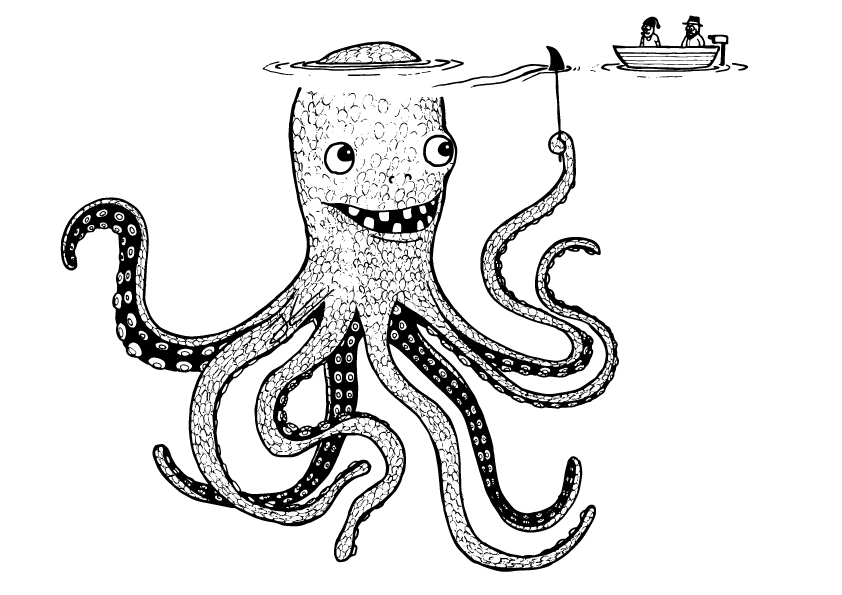
\includegraphics[width=0.9\textwidth,natwidth=842,natheight=595]{./imagens/octupus.jpg}
\end{center}
\end{slide}


\end{document}
\endinput